% This is samplepaper.tex, a sample chapter demonstrating the
% LLNCS macro package for Springer Computer Science proceedings;
% Version 2.21 of 2022/01/12
%
\documentclass[runningheads]{llncs}

% for links
\usepackage{hyperref}
\hypersetup{
    colorlinks=true,
    linkcolor=blue,
    filecolor=magenta,      
    urlcolor=cyan,
    pdftitle={Overleaf Example},
    pdfpagemode=FullScreen,
    }
%
\usepackage[T1]{fontenc}
% T1 fonts will be used to generate the final print and online PDFs,
% so please use T1 fonts in your manuscript whenever possible.
% Other font encondings may result in incorrect characters.
%
\usepackage{graphicx}
% Used for displaying a sample figure. If possible, figure files should
% be included in EPS format.
%
% If you use the hyperref package, please uncomment the following two lines
% to display URLs in blue roman font according to Springer's eBook style:
%\usepackage{color}
%\renewcommand\UrlFont{\color{blue}\rmfamily}
%
\begin{document}
%
\title{Complexity in Boardgames}
%
%\titlerunning{Abbreviated paper title}
% If the paper title is too long for the running head, you can set
% an abbreviated paper title here
%
\author{Marco Luzzara\inst{1}\orcidID{0000-0002-6414-3727}}
%
% First names are abbreviated in the running head.
% If there are more than two authors, 'et al.' is used.
%
\institute{Università Degli Studi di Milano}

%
\maketitle              % typeset the header of the contribution
%
\begin{abstract}
In this paper, I have analyzed the complexity in the board games and the factors that can increase it. boardgamegeek.com (BGG), a popular website for boardgames fans, has assigned a complexity score, called weight, to each boardgame. The purpose of this project is to predict the complexity of a boardgame, starting from the data found on BGG, like rulebooks and playing time. I have extracted them using the BGG APIs, then I have processed them with Python and some NLP libraries, like Spacy and Coreferee. Eventually, I have used Scikit-Learn to find the best model that predicts the game complexity.
I have found that the factors that mostly determines the complexity are the playing time, the rulebook length, the family of the game and the number of entities the game presents.
The biggest issue I have with the current model is the amount of outliers, caused by mainly 2 reasons. The first one is the data retrieval algorithm, which is not always able to retrieve the correct rulebook. The second one regards the relationship between depth and complexity. While it is possible to measure the complexity of a board game, evaluating its depth is harder using only the data retrieved.

\keywords{Boardgame \and Complexity \and Weight}
\end{abstract}
%
%
%

\section{What Is Complexity and Why It Differs From Depth}
The complexity of a game is a difficult concept to define and it often intersects with the concept of depth. 

\subsubsection{Complexity}
A game is complex when the rules have many interactions with each other. According to this definition, a game with a few rules might be as complex as a game with a lot of rules. Basically, the number of rules do not affect the complexity of a game, only the amount of interactions between rules affects it.

\subsubsection{Depth}
The depth of a game is the sum of each decision's depth. A decision is depth when it can generate many possible outcomes throughout the game. A decision can bring to other decisions as well, that is why depth is highly related to the decisions' ramification.  \\

\textit{Chess}, for example, is a very deep game, but not complex at all. A decision in chess, like moving a pawn, opens an infinite number of possibilities. On the other hand, there are not many rules (at least the basic ones) that "interact" with the others, so Chess is not a complex game. \\

BGG has a metric called \textbf{Weight}, a float between 1 and 5 that is the average of the users' votes of complexity. To evaluate it, each user is supposed to take into consideration \href{https://boardgamegeek.com/wiki/page/Weight}{many factors}. These criteria have both complexity and depth components. In particular, the \textit{amount of choices available} is a clear reference to depth. \\
In this project, I have assigned a score to most criteria and used them in a predictive model to get as close as possible to the BGG weight. I have focused on complexity, whereas depth is a difficult metric to evaluate with the data I have gathered. It is usually a property of the game that cannot be inferred only from the rules. 

\section{Data Retrieval}
\subsection{BoardGameGeek APIs}
\href{https://boardgamegeek.com}{BoardGameGeek} is a website that provides some \href{https://boardgamegeek.com/wiki/page/BGG_XML_API2}{public APIs} to retrieve information on board games. The information I have queried are the playing time, the categories that a board game belongs to and the weight. I have queried this metric together with the number of votes sent by the users to subsequently filter the board games with too few votes. The APIs do not allow the rulebooks' download, so I had to use several internal APIs, which are not documented. 

\subsection{Dataset Building}
\subsubsection{Rulebook Download}
In the BGG page for a board game, there might be many files, not necessarily only the rulebook. In order to avoid unreadable files, I have decided to search for the top 25 PDF files written in english. Instead of downloading all of them, I have used a very simple search engine based on Tf-Idf to get the file most similar to a rulebook. The documents used in the Tf-Idf engine are the file descriptions and the similarity metric is the cosine similarity. This is the query:

\begin{verbatim}
"revised official rule rulebook update new"
\end{verbatim}

\noindent After some tries, I have noticed that these ones are the most frequent words in a rulebook's description. Then, I have downloaded the target file and used PyMuPDF to read it. In order for a file to be accepted, it must:
\begin{itemize}
    \item Contain at least 1 letter.
    \item Contain at least 10 periods (10 sentences)
\end{itemize}

\noindent These checks are necessary because the rulebooks of some boardgames are not publically available or the PDF parser is not able to get the written content. This usually happens when some rules are shown as images.
These checks are simple but quite efficient to filter the garbage files. However, I had to manually review the accepted files because some rulebooks were clearly uncomplete or were multi-language. Improving the rulebook's retrieval process is one of the main challenges of this project.

\subsubsection{Data Filtering}
Aside from the conditions above, there are other checks a boardgame must pass in order to become part of the dataset:

\begin{itemize}
    \item The playing time, the weight and the rulebook must be present. Instead, the category is not strictly necessary. The number of votes for the weight is always present if the weight is present.
    \item The votes for the weight must be more than 10.
\end{itemize}

\noindent The dataset is a CSV file containing the fields described in Table 1.

\begin{table}
\caption{Dataset fields}\label{tab1}
\begin{tabular}{|l|l|}
\hline
Field Name & Description\\
\hline
\verb|rulebook| & The boardgame rulebook \\
\verb|id| & The BGG Id of the boardgame \\
\verb|name| & The boardgame name \\
\verb|averageweight| & The average of the complexity scores given by the user \\
\verb|playingtime| & The playing time \\
\verb|family| & List of the boardgame's categories, like family game, strategy, etc \\
\hline
\end{tabular}
\end{table}

\section{Data Preprocessing}
The \textit{playingtime} in the above fields remains unchanged because it is already a feature. The \textit{rulebook} and \textit{family} fields must be processed.

\subsection{Family Field Processing}
The \textit{family} field is stored in the CSV as a list of strings. The reason is that a boardgame could belong to many families. I have used Pandas to convert it to a \verb|DataFrame| with the single families as columns. For example, these lists

\begin{verbatim}
1. ["familygame", "strategy"]
2. []
3. ["abstract", "strategy"]
\end{verbatim}

\noindent Are converted to as shown in Table 2.

\begin{table}
\caption{Families one-hot encoding}\label{tab2}
\begin{tabular}{|l|l|l|l|}
\hline
familygame & strategy & abstract & unspecified\\
\hline
1 & 1 & 0 & 0 \\
0 & 0 & 0 & 1 \\
0 & 1 & 1 & 0 \\
\hline
\end{tabular}
\end{table}

The new \verb|DataFrame| has as many columns as the number of families encountered during the one-hot encoding process. The row values of each boardgame are 1 or 0 depending on the presence of that family in the \textit{family} list. \textit{unspecified} is a special value used when the family type is missing (BGG does not fill it).

\subsection{Rulebook Cleaning}
Firstly, rulebooks need a cleaning phase because the PDF parsing is typically very imprecise. In this part, I have used multiple regex to:
 
\begin{itemize}
    \item Remove mails and HTTP links
    \item Make tokenization more accurate 
    \item Remove rules references (e.g. 1.2.3)
    \item Recover missing apices (e.g. \textit{can t} $\rightarrow$ \textit{can't})
    \item Drop sentences that has less than a minimum number of words
\end{itemize}

\subsection{Rulebook Preprocessing}
The rulebook processing part is also based on finding the main entities that contribute to add complexity to the game. In order to do this, pronouns and references are replaced with the entities they refer to. This was necessary because the metrics I have computed depend on the word frequencies and their position in the text. This operation is called \textbf{coreference resolution}. For example, this sentence

\begin{verbatim}
    Although he was very busy with his work,
    Peter had had enough of it.
\end{verbatim}

\noindent Is converted to

\begin{verbatim}
    Although Peter was very busy with Peter work, 
    Peter had had enough of work.
\end{verbatim}

\noindent The library I have used is \href{https://explosion.ai/blog/coref}{coreferee} and it perfectly integrates with Spacy.

\section{Rulebook Feature Extraction}

\subsection{Luck Score}
The first criterion I have analyzed to predict a boardgame weight is the amount of luck present in the game. I have identified these main sources of luck:

\begin{itemize}
    \item Drawing a card/tile/etc
    \item Shuffling a deck
    \item Rolling a die
\end{itemize}

\noindent These actions are very frequent in boardgames and easily recognizable in the rulebook as well. Spacy provides a dependency matcher that searches the specified patterns in the text. These patterns are built using the tokens' part of speech and the dependencies they have with the other tokens. Another "pattern" I have included in the search is "random/randomly". For all of these actions, the player does not have to make a choice, because the consequences of these actions are independent from the player himself. What a player does not control should not be defined as complex/deep. The absence of a choice makes the game more linear.
\\
Another possible source of luck is the flipping of a coin/card, but that is commonly used at the game start to decide who is the first player. This does not affect the game complexity, so I have not included it in the score.

The number of matches found for each of these actions are then normalized using the rulebook length. 

\subsection{Amount of Available Choices}
This score is probably the most complex to compute because it is a property of the game that can be discovered exclusively by playing it. The approach I have used is very similar to the previous one, with the Spacy dependency matcher. In this case, the patterns match when I find:

\begin{itemize}
    \item \textit{can}, \textit{could} or \textit{may}, in the positive form, but not next to \textit{only} or \textit{never}. 
    \item \textit{decide}, \textit{select}, \textit{choose} or \textit{opt}, not preceded by a modal verb and with the same constraints as in the above pattern.
    \item \textit{choice} and \textit{option}, not preceded by \textit{no} (e.g. \textit{no option} means the player does not have a choice)
\end{itemize}

\subsection{Entities Search}
An entity can be the game material, as well as an abstract component, like a resource type in a \href{https://en.wikipedia.org/wiki/Eurogame}{Eurogame}. The parameters used to extract the entities are:

\begin{itemize}
    \item An entity is a noun that has at least 3 characters and have at least 4 occurrences in the rulebook.
    \item \verb|token.dep_ in {'nsubj', 'nsubjpass', 'dobj'}| at least once.
    \item The minimum distance between two tokens of the same entity must be lower than a threshold. This is to avoid that common nouns are included among the entities.
\end{itemize}

\noindent Entity extractions is a difficult task because its definition is not clear. Even considering an entity as something that generically increases the game complexity, we still have some issues that have not been covered. The first problem is the presence of synonyms: the same entity could be named differently. Fortunately, this does not usually happens. 

Two other possible approaches to find entities are keyword extraction and entity recognizer. I did some tests using rake and yake, two keyword extraction algorithms, but the results were unsatisfactory. Spacy has an entity recognizer integrated in the pipeline, but that is not suitable here because it tends to recognize only proper names.

\subsection{Actions Score}
Each entity can have many actions associated. These actions are translated to verbs in the rulebook. This score is simply the number of different verbs associated to the entities over the number of entities. 

\subsection{Lexical Diversity}
Lexical diversity expresses the ratio of different unique words over the total number of words. A rulebook having a rich lexicon is more likely to be complex. Many different lexical diversity scores exist, but I needed one that does not depend on the text length and with a high sensitivity. 
The paper \textit{Lexical Statistics and Tipological Structures: A Measure of Lexical
Richness}~\cite{lexical_richness} studies and compares a lot of indexes and the one that better fits in this context is the \textbf{MTLD} (Measure of Textual Lexical Diversity).

I have used a python package called \verb|lexicalrichness| that already has an implementation for MTLD. 

\subsection{Interactions Score}
This score is probably the nearest to the definition of complexity given at the start. Instead of analysing the interactions of rules, my interactions score considers the entities. Two entities interact with each other when they are present in the same sentence. I have then built a matrix where each cell contains the number of sentences shared by both the entities involved. This matrix represents the sparse graph of interactions, on which I compute the network density metric:\\

$ InteractionScore = \frac{2 * matrix.sum()}{len(entities) * (len(entities) - 1)} $ \\

\noindent For example, with this matrix:

\begin{verbatim}
                player      card        warrior
    player      0           2           4       
    card        0           0           3
    warrior     0           0           0
\end{verbatim}

\noindent The \verb|InteractionScore| would be 3.

\subsection{Entity variance}
The variance of an entity expresses how much an entity is sparsed in the rulebook. It can be useful because when an entity variance is high, then there are many points in the rulebook where we need to consider it. The total variance is computed as:

$\frac{\sum_{i = 0}^{len(entities)} \frac{len(tokens_i)}{len(all\ tokens)} * np.var([token.sentence\_id\ for\ token\ in\ tokens_i])}{len(sentences)} $

\section{Weight Prediction}
The previous features are gathered in a \verb|DataFrame| and processed using the models that \verb|scikit-learn| library provides.

\subsection{Training}
I have split the features set into train and test sets. I have used \verb|GridSearchCV| for hyperparams tuning and simple cross-validation to collect the train set metrics. As for the preprocessing phase, I needed a scaler robust to outliers, that is \verb|RobustScaler|. 

Regarding the feature selection, I have used \verb|RFECV| for models based on coefficients, like the \verb|LinearRegression|, \verb|Lasso| and \verb|Ridge|. For the other models, except for decision trees based ones, I have used \verb|SelectKBest|, and found the \verb|k| parameter during hyperparams tuning.

For each tested model, I have computed the \textit{R2}, \textit{Mean Absolute Error (MAE)}, \textit{Mean Absolute Percentage Error} and \textit{Mean Squared Error} metrics, and ordered the results by \textit{MAE}. The models with the better results are, in descending order, the \verb|SVR|, \verb|KNeighborsRegressor| and \verb|ExtraTreesRegressor|. All of them have a \textit{MAE} less or equal than \verb|0.32|. Figure~\ref{fig1} is a plot created using \verb|PredictionErrorDisplay| for the \verb|SVR| model.

\begin{figure}
    \centering
    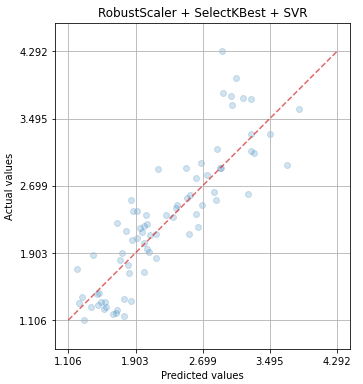
\includegraphics[width=0.39\textwidth]{images/SVR_Predictions.png}
    \caption{Visualization of the prediction error for the SVR model} \label{fig1}
\end{figure}

\clearpage

\subsection{Results Analysis}
The generalization error is around 0.30, but only few of the features previously found are relevant. Among the most useful features, there are the playing time, the game family (like strategy game, party game, etc), the entities count and variance and the rulebook length. Among these features, the playing time is definitely the most important one. The interactions score is sometimes included in the features selected by the KBest selector. The permutation importance analysis gives some interesting insights on the features importance. 

\begin{verbatim}
    Selected features: ['playingtime', 'rulebook_len', 
        'entities_count', 'interaction_score', 'entities_variance',
        'actions_score', 'familygames', 'strategygames']
    
    Permutation Importance of 1 out of 5 SVR estimators trained:
    playingtime         0.664 +/- 0.045
    rulebook_len        0.150 +/- 0.017
    strategygames       0.146 +/- 0.014
    entities_count      0.107 +/- 0.011
    entities_variance   0.095 +/- 0.010
    familygames         0.063 +/- 0.008
    actions_score       0.036 +/- 0.006
\end{verbatim}

Metrics computed through pattern matching turn out to be weak compared to the others. The lexical richness is another feature that does not affect the weight to a significant extent. 

\section{Future Work}
The biggest issue I have found is related to data reliability. Many of the rulebooks I have downloaded are incomplete, poorly parsed or not even rulebook. Some rulebooks are just a sequence of Q/A, others describe some variations of the original game. A better rulebook selection and cleaning process would probably decrease the amount of outliers.

The second improvement that can be done is evaluating the depth of the game. The BGG weight of a depth game is usually very high. Chess weight is 3.67, but it is difficult to predict it using only the rulebook. It would certainly be useful to process different types of resources, like "cheatsheet", Q/A, manuals and whatnot.

The entities count and variance seem two promising scores. Improving the algorithm to find the entities could greatly increase the model accuracy.

%
% ---- Bibliography ----
%
% BibTeX users should specify bibliography style 'splncs04'.
% References will then be sorted and formatted in the correct style.
%
% \bibliographystyle{splncs04}
% \bibliography{mybibliography}
%
\begin{thebibliography}{8}
\bibitem{keyword_extraction}
Eugenia Spano: Keyword Extraction and Classification - (2018)

\bibitem{lexical_richness}
Joan Torruella, Ramon Capsada: Lexical Statistics and Tipological Structures: A Measure of Lexical
Richness - (2013) 447 – 454
\end{thebibliography}
\end{document}
